\section{Key-value database}

Key-value databases store data as a collection of key-value pairs. 
This structure allows for efficient retrieval of data. 
Conceptually, the key-value approach is analogous to indexing in relational databases, where a key serves as a reference to access the associated data object.

\subsection{Redis}
Redis supports atomic operations on its native data structures, ensuring that operations on a specific data type can be completed without interference from other operations. 
Redis can be used as a persistent database, a fast in-memory cache, or a message broker, making it a multi-purpose tool in modern architectures. 

While Redis is not a direct replacement for relational databases or document stores, it complements them well. 
Best use cases for Redis are: 
\begin{itemize} 
    \item Applications that require real-time data processing and fast access.
    \item Scenarios needing complex data structures, such as lists and sets, rather than basic key-value pairs.
    \item Situations where the dataset fits within memory, allowing for fast in-memory data retrieval.
    \item Non-critical datasets, as Redis persistence mechanisms can introduce some latency, which may be unsuitable for mission-critical applications.
\end{itemize}
\noindent The advantages of Redis are: 
\begin{itemize}
    \item \textit{Performance}: Redis offers high-speed data access, ideal for real-time applications.
    \item \textit{Availability}: replication and partitioning enhance data availability and fault tolerance.
    \item \textit{Scalability}: Redis can be scaled to accommodate high-demand scenarios.
    \item \textit{Portability}: Redis runs on most POSIX-compliant systems and has limited support for Windows.
\end{itemize}

\subsubsection{Architecture}
Redis, written in C, runs on most POSIX-compliant systems, with Linux recommended for production environments. 
Although Redis is single-threaded, it achieves scalability across multiple CPU cores by allowing multiple Redis instances to run in parallel. 
With constant-time complexity for many commands, Redis remains efficient even with high data volumes.
\begin{figure}[H]
    \centering
    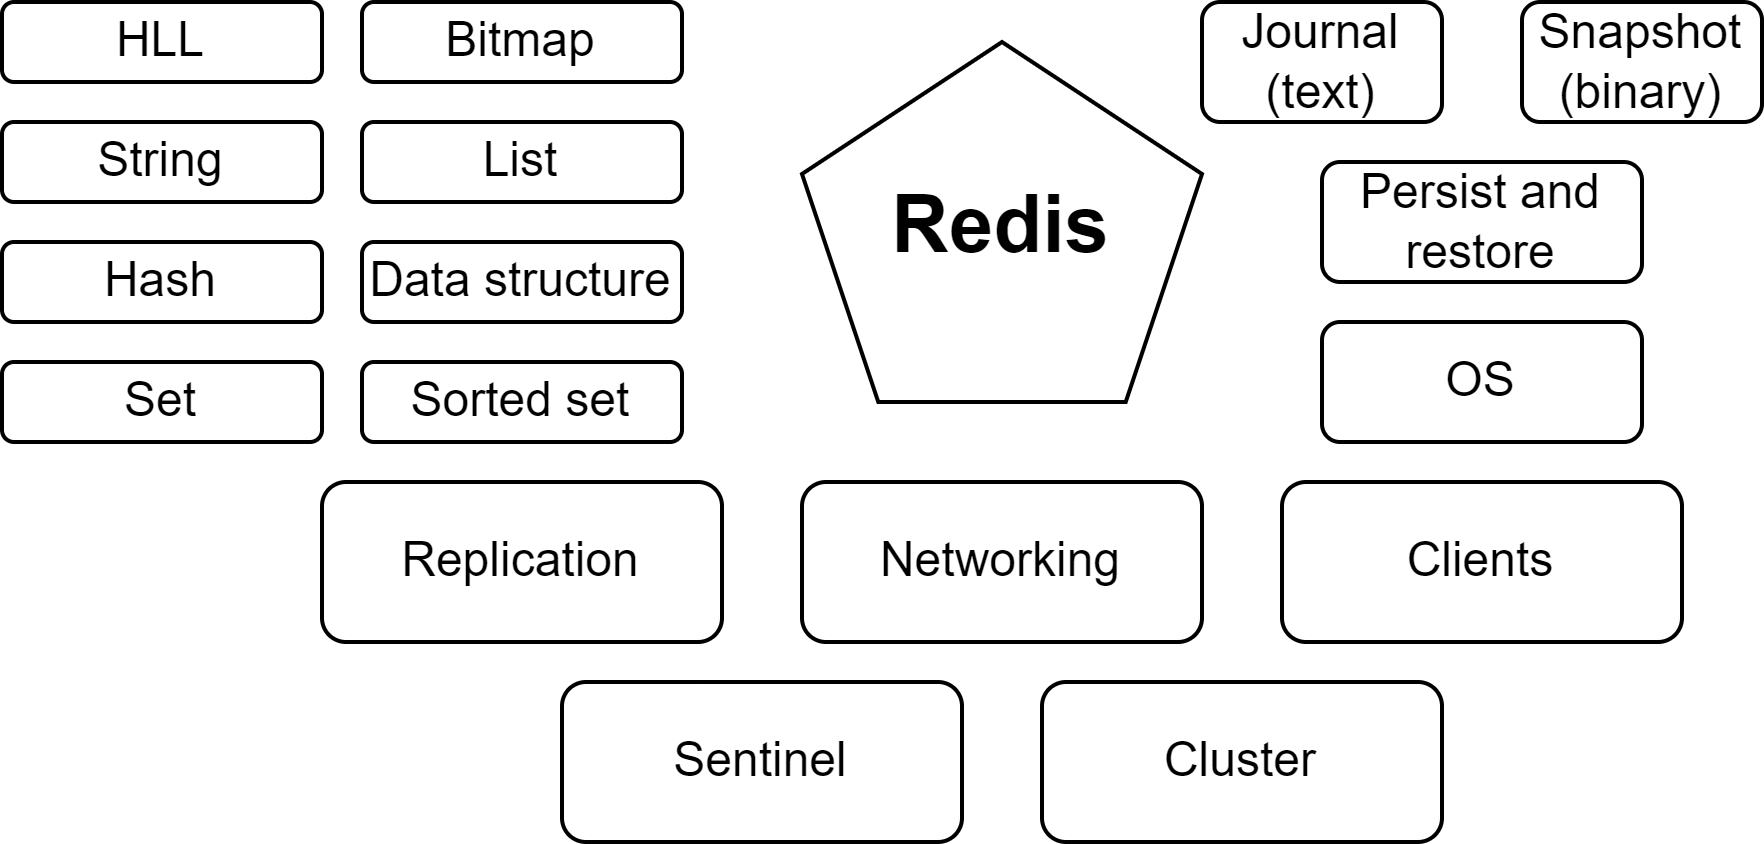
\includegraphics[width=0.75\linewidth]{images/redis.png}
    \caption{Redis architecture}
\end{figure}
\noindent Redis offers two persistence mechanisms:
\begin{itemize}
    \item \textit{Redis Database Snapshots}: captures a snapshot of the dataset at specified intervals.
    \item \textit{Append-Only File}: logs every write operation, ensuring recovery by replaying commands if Redis restarts.
\end{itemize}
Redis enables master-slave replication, where one master Redis instance can synchronize with multiple read-only slave instances. 
Clients can read data from both master and slave nodes, but only write to the master by default. 
Redis also supports data partitioning across multiple hosts through:
\begin{itemize}
    \item \textit{Client-side partitioning}: client code manages data distribution.
    \item \textit{Proxy-based partitioning}: uses a proxy layer to distribute requests.
    \item \textit{Query router partitioning}: Redis Cluster automatically routes requests to the appropriate node.
\end{itemize}

\paragraph*{Cofigurations}
Redis can be deployed in various configurations:
\begin{itemize}
    \item \textit{Standalone}: basic setup with optional master-slave replication for read offloading and redundancy. 
        No automatic failover.
    \item \textit{Sentinel}: provides automated failover in a master-slave topology, promoting a slave to master if the primary fails. 
        Data is not distributed across nodes.
    \item \textit{Twemproxy}: functions as a proxy to distribute data across standalone Redis instances, supporting consistent hashing and basic partitioning.
    \item \textit{Cluster}: Redis Cluster distributes data across multiple instances with built-in failover and divides the keyspace into hash slots, where each node holds a subset of the hash slots.
\end{itemize}

\subsubsection{Data model}
The Redis data model is centered around key-value pairs, with additional data types for more complex storage needs.
\begin{table}[H]
    \centering
    \begin{tabular}{|c|l|}
    \hline
    \textbf{Data type} & \textbf{Description} \\ \hline
    \textit{Strings}            & Basic key-value pairs, suitable for caching and counters \\ \hline
    \textit{Lists}              & Ordered collections, useful for queues \\ \hline
    \textit{Sets}               & Unordered unique collections, great for tags and unique items \\ \hline
    \textit{Sorted sets}        & Sets with key, ideal for rankings \\ \hline
    \textit{Hashes}             & Field-value pairs within a key, good for storing objects \\ \hline
    \textit{Bitmaps}            & Bit-level data, useful for flags and tracking events \\ \hline
    \textit{HyperLogLogs}       & Probabilistic unique counters with low memory usage \\ \hline
    \textit{Streams}            & Log-like data for real-time processing and event sourcing \\ \hline
    \end{tabular}
\end{table}

\subsubsection{Query language}
Redis uses a command-based language tailored to its data types. 
Commands are specific to the type of data being manipulated, ensuring efficient data access and manipulation for diverse data structures.

\paragraph*{Strings}
The basic commands on strings are: 
\begin{lstlisting}[style=Redis]
/* get and set strings */
SET string_key string_value
GET string_key 
/* set or increment numbers values */
SET string_key 1
INCRBY string_key 1
/* get and set multiple keys at once */
MGET string_key string_key
MSET string_key string_value
/* get the length of a string */
STRLEN string_key 
/* update a value retrieving the old one */
GETSET string_key string_value
\end{lstlisting}

\paragraph*{Keys}
The basic commands on keys are: 
\begin{lstlisting}[style=Redis]
/* key removal */
DEL key_value
/* test for existence */
EXISTS key_value
/* get the type of a key */
TYPE key_value
/* set an expiration time to a key */
EXPIRE key_value 10 
/* get key time-to-live */
TTL key_value
\end{lstlisting}

\paragraph*{List}
The basic commands on list are: 
\begin{lstlisting}[style=Redis]
/* push on either end */
RPUSH key_value string
LPUSH key_value string
/* pop from either end */
RPOP key_value
LPOP key_value
/* blocking pop on either end */
BRPOP key_value
BLPOP key_value
/* pop and Push to another list */
RPOPLPUSH src_key_value dst_key_value
/* get an element by index on either end */
LINDEX key_value
/* get all list elements */
LRANGE key_value 0-1
\end{lstlisting}

\paragraph*{Hash}
The basic commands on hash are: 
\begin{lstlisting}[style=Redis]
/* set a hashed value */
HSET key:key_value field value 
/* set multiple fields */
HMSET key:key_value lastfield Smith visits 1
/* get a hashed value */
HGET key:key_value field
/* get all the values in a hash */
HGETALL key:key_value
/* increment a hashed value */
HINCRBY key:key_value visits 1
\end{lstlisting}

\paragraph*{Sets}
The basic commands on sets are: 
\begin{lstlisting}[style=Redis]
/* add member to a set */
SADD key value
/* pop a random element */
SPOP key
/* get all elements */
SMEMBERS key
/* intersect multiple sets */
SINTER key key
/* union multiple sets */
SUNION key key
/* differentiate multiple sets */
SDIFF key key
\end{lstlisting}

\paragraph*{Sorted sets}
The basic commands on sorted sets are: 
\begin{lstlisting}[style=Redis]
/* add member to a sorted set */
ZADD key key_value value
/* get the rank of a member */
ZRANK key value
/* get elements by score range */
ZRANGEBYSCORE key 200 +inf WITHSCORES
/* increment score of member */
ZINCRBY key 10 value 
/* remove range by score */
ZREMRANGEBYSCORE key 0 key_value
\end{lstlisting}

\subsection{Memcached}
Memcached is an open-source, distributed memory caching system created in 2003 by Brad Fitzpatrick to boost the performance of dynamic web applications by reducing database load. 
Using a key-value dictionary model, Memcached is particularly useful for storing frequently accessed, computationally expensive, or commonly shared data in memory, allowing applications to access it quickly. 
Originally intended to speed up dynamic websites like LiveJournal, Memcached is now widely used to cache data temporarily, ensuring faster response times without putting undue strain on databases.

Technically, Memcached operates as a server that clients can access over TCP or UDP, and multiple Memcached servers can be grouped into pools to expand available cache memory. 
This setup allows for a high degree of flexibility and scalability, particularly in large applications where caching demands are extensive.

In practice, Memcached excels when caching frequently accessed data. 
Typical uses for Memcached include caching key session values and data, which are both accessed often and shared widely.
It's also ideal for storing homepage data, which is computationally expensive and frequently accessed, making it crucial for optimal load times.

Caching at a lower level, as with Memcached, effectively reduces load on databases, which often constitute the main performance bottleneck in backend systems. 
By handling many database requests at the memory level, Memcached accelerates response times and offloads work from the database.

Memcached employs a simple invalidation strategy by setting expiration times on cached items, allowing data to automatically expire rather than requiring manual deletions. 
This approach can result in slightly outdated data, which is acceptable for summaries, overviews, and other low-criticality pages. 
For high-sensitivity data, however, it's possible to set up conditional expiration.

Although it reduces database requests, each Memcached call still has a performance cost.
To mitigate this, techniques like multi-get can retrieve multiple keys in a single call, reducing response time by returning an array of items. 
Security is another consideration, as early versions of Memcached had no built-in authentication. With the addition of the SASL Auth Protocol, securing access to Memcached has become easier.